\chapter{基于深度强化学习混合模型在直复营销中的研究}
自从DeepMind团队提出DQN模型之后,掀起了研究深度强化学习的高潮。因为在复杂的现实应用中,DQN模型通过神经网络强大的非线性表征能力,可以进行状态特征的自动提取,进而更好的逼近值函数。所以,在本章中,针对直复营销场景中客户状态的部分可观测问题,提出使用基于RNN的深度强化学习的方法(RNN_DQN)进行解决。特别地,为了更好的学习隐状态的表征方法,对RNN_DQN模型从网络结构和训练方法上提出了不同的改进方法。

\section{研究动机}
\subsection{状态的部分可观测性与线性函数逼近}
在马尔科夫决策过程中,要求系统的状态具有马尔科夫性,即下一个时刻的状态$S_{t+1}$仅与当前的状态$S_{t}$和当前要采取行为$A_{t}$有关,与系统之前所拥有的状态和采取的行为都无关。因为强化学习是建立在马尔科夫决策过程基础上的,所以,当采用强化学习对直复营销场景进行建模时,存在的一个前提假设是:客户的当前状态应该完全概括了他与营销人员在此之前的整个交互历史。也就是说,客户下一时刻的响应情况仅与他当前的状态和营销人员下一时刻要采取的营销行为有关,与之前的交互历史都无关。但是,和很多其他现实应用所面临的问题一样,在直复营销场景中,因为客户的状态存在部分可观测性(Partial Observability)的问题,使得上述这个假设很难得到满足。

在本文的第三章中,为了更好的捕捉募捐者的状态,在进行仿真实验的时候,从募捐者的观测数据中人工提取了大量的中间特征,而这些特征有很多是需要借助专家领域知识或者经验才能获得的。即便如此,这也只概括了募捐者真实状态中的部分信息。因此,在对这些存在状态部分可观测问题的应用场景使用强化学习之前,进行状态的推断学习是很重要的。

在强化学习的研究和应用中,处理部分可观测问题最常用的方法有两种,其一是使用部分可观测的马尔科夫决策过程(Partially Observable Markov  Decision Process,POMDP)\citep{kaelbling1998planning},其二是预测状态表示法(Predictive State Representation,PSR)\citep{littman2002predictive}。POMDP虽然有着坚实的理论基础,并且已经在一些诸如机器人、人机对话等领域取得了不错的表现\citep{pineau2003point,williams2007partially},但是POMDP模型的建立需要依赖部分可观测的名义状态(Nominal State),所以系统的POMDP是很难学习的,而且还需要很多专家的先验知识来定义隐藏状态集和观测概率集。于是,Littman等人于2002年提出了一种新的动态系统建模方法——PSR\citep{littman2002predictive},用于处理部分可观测的问题,PSR的优势在于仅通过观察值序列就可以预测未来事件。尽管PSR具有很强的表示能力,并且比POMDP方法更容易从数据中学到信息,但是仍然需要大量的领域知识来设计特征和核函数。所以,在直复营销这类复杂的现实应用中,构建具有马尔科夫性的状态来解决部分可观测的问题是很难的。

另外,为了保证值函数的收敛性,本文第三章所提出的算法均选择了参数化线性函数逼近的方法。但是,由于在线性函数逼近方法中,基函数的个数是需要事先固定的,导致其表征能力非常有限,对于复杂的问题,数量太少的基函数无法得到好的逼近效果,并且函数的形式是也是需要事先选定的的,这也限制了函数的逼近能力。

\subsection{深度强化学习}
近年来,强化学习和深度神经网络的结合取得了重大突破,并成功的应用在了游戏、围棋等领域\citep{mnih2013playing, mnih2015human},形成了一个重要的研究方向:深度强化学习。深度强化学习在现实应用中之所以会取得如此令人振奋的表现,除了充分发挥了强化学习技术在序贯决策上的优势外,还离不开神经网络的强大作用。

具体地,神经网络在强化学习中的作用主要包括两个方面:一方面,利用了神经网络强大的非线性逼近能力进行值函数的逼近,以更好的学习最优策略;另一方面,神经网络在训练的过程中,可以自动的进行状态特征的学习和表示,在一定程度上解决状态的部分可观测问题。另外,与上述POMDP和PSR方法不同,基于神经网络的方法可以在不依靠专家领域知识的情况下,对任何问题都可以给出状态特征的合理表示方法\citep{deng2014deep},从而解决了在实际应用中,需要人为设计状态特征的困扰。

受此启发,本文提出使用深度强化学习的方法来解决直复营销的决策问题。期望通过神经网络的方法可以在提高值函数逼近精度的同时,能更好解决直复营销场景中的客户状态的部分可观测问题,特别地,本章重点关注针对后者的优化。具体来说,本章从深度强化学习DQN模型出发,结合直复营销场景的时序特点,提出使用基于循环神经网络的DQN模型(DQN_RNN)来更好的解决上述问题。另外,在强化学习的过程中,为了保证在进行值函数逼近的同时不影响隐状态学习,本文提出了基于RNN的深度强化学习混合模型,并对的网络结构进行了进一步的分析和优化。

需要特别说明的是,为了进行更优针对性的研究,本章决定简化问题的复杂度,暂不考虑营销中的可变时间间隔问题,而只关注于定期营销策略的研究。


\section{DQN_RNN模型}
因为本章所提出的改进模型是基于DQN模型的,所以为了更好的理解后续所研究的内容,本节中首先对DQN模型的学习过程进行介绍,并分析其在处理序列问题上的不足,然后介绍RNN网络的特点进而引出DQN_RNN模型。另外,在本节中,将提到的DQN模型和DQN_RNN模型作为本章试验对比基准模型,并对其如何应用到直复营销场景中进行了简单介绍。

\subsection{DQN模型}
如第二章所述,在强化学习中,当使用参数化非线性函数(神经网络)逼近的方法逼近值函数的时候,因为数据样本之间的相关性,往往会造成值函数不收敛的问题。为了解决这个问题,2013年,谷歌(Google)的DeepMind团队提出了DQN模型,并于2015年对DQN进行了进一步优化,将其成功的应用在了围棋和游戏上。DQN模型是在传统的Q-learning算法($\ref{algo:algorithm_2}$)的基础上改进而来,如第二章所述,DeepMind团队主要从以下三个方面进行了改进:
% \begin{itemize}
% \item 使用卷积神经网络进行Q值函数的逼近。
% \item 通过经验回放(Experience Replay)机制来解决强化学习中相关性以及非静态分布的问题。
% \item 通过独立设置目标网络(Target Net)来单独处理时间差分算法中的TD偏差,进一步降低数据之间的关联性,从而削弱收敛不稳定的问题。
% \end{itemize}

(A)、使用卷积神经网络CNN进行Q值函数的逼近。

(B)、通过经验回放(Experience Replay)机制来解决强化学习中样本之间的相关性以及样本的非静态分布的问题。

(C)、通过独立设置目标网络(Target Net)的方式,来单独处理时间差分算法中的TD偏差,进一步降低数据之间的关联性,从而削弱值函数收敛不稳定的问题。

 为了更好的介绍本节提出的改进模型,接下来本章将结合DeepMind团队发表的文献\citep{mnih2013playing,mnih2015human}来分析DQN模型的学习过程:

\paragraph{DQN模型的学习过程}
根据文献\citep{mnih2015human}中作者提供的DQN模型伪代码,本节首先绘制出了DQN模型的流程图(如图$\ref{fig:liuchengtu_DQN}$所示),并总结出了DQN模型的学习过程主要包括以下几步:
 % 从文献中可以得到DQN模型的伪代码如所示。根据算法$\ref{algo:algorithm_DQN}$,

\begin{figure}[htbp]
\centering
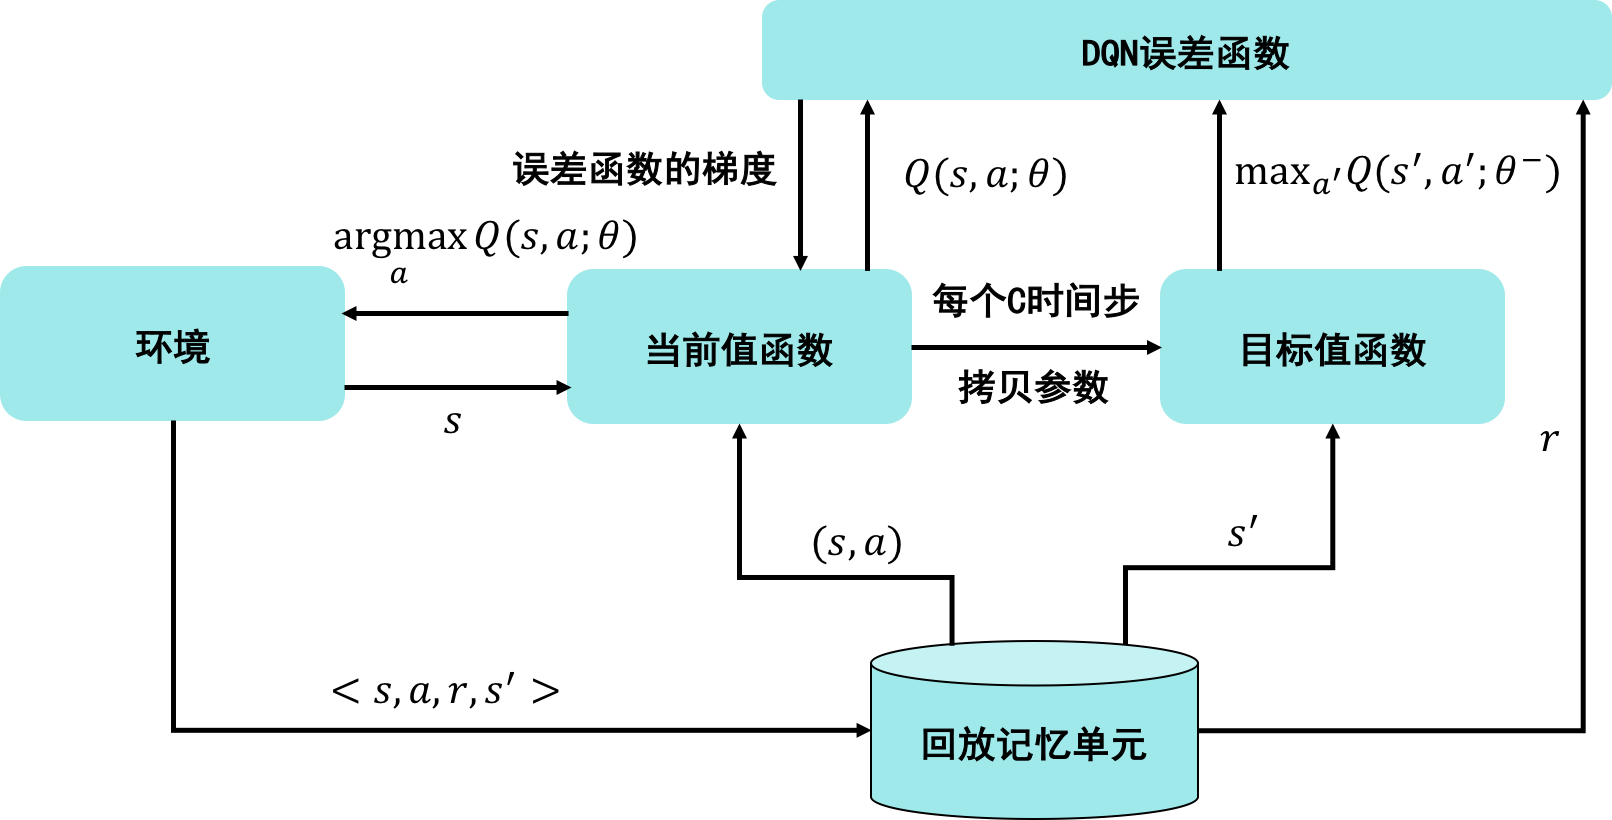
\includegraphics[width=1.0\textwidth]{liuchengtu_DQN1}
\caption{DQN模型的流程图}
\label{fig:liuchengtu_DQN}
\end{figure}
 
(A)、构建回放记忆单元。首先,初始化状态$s$,然后,在接下来的每个时间步里,按照$\epsilon-greedy$策略选择行为$a$,并在仿真器中执行$a$,即可得到对应的即时奖赏$s$和下一步的状态$s^{'}$,将此转换样本$<s, a, r, s^{'}>$放到回放记忆单元中。

(B)、值函数的学习(即当前值网络MainNet的参数更新)。从回放记忆单元中随机选取一小批转移样本,并使用当前值网络(MainNet)和目标值网络(TargetNet)分别计算出Q估计值 $Q(s,a;\bm{\theta})$和Q目标值$r+\gamma \max_{a^{'}}Q(s^{'},a^{'};\bm{\theta}^{-})$,然后通过均方误差的方式得到损失函数$L=[r+\gamma \max_{a^{'}}Q(s^{'},a^{'};\bm{\theta}^{-})-Q(s,a;\bm{\theta})]^{2}$,并使用随机梯度下降法(如公式$\eqref{dituxiajiangq}$所示)进行当前值网络(MainNet)的参数更新。
% $<S_{j}, A_{j}, R_{j}, S_{j+1}>_{j=1}^{N}$

(C)、更新目标值网络(TargetNet)参数。经过若干步的训练后,将当前网络的参数拷贝给目标值网络,进行目标值网络的参数更新。 

(D)、当DQN模型训练完毕后,将环境的当前状态$s$输入到当前值网络,DQN模型便会输出的动作选择策略$\pi(s)=\argmax_{a}Q(s,a;\bm{\theta})$。

\paragraph{DQN模型的损失函数}
进一步地,为了更好地了解DQN模型的参数更新过程,可以将DQN模型的损失函数构建过程表示为图$\ref{fig:loss_DQN}$的形式,从图$\ref{fig:loss_DQN}$中可以看出,当前值网络(MainNet)和目标值网络(TargetNet)都是以状态$s$作为输入,并且输出的是各行为的Q值。其中,当前值网络的简化构造如图中左侧部分所示,DQN模块是一个CNN网络,需要特别注意的是,在当前值网络的训练过程中,前一个输出和后一个输入之间是没有关系的。

在构建损失函数时,首先将状态$s$输入到当前值网络,并根据行为$a_{i}$($a_{i}$表示离散行为的类型)从当前值网络找到对应的Q估计值$Q(a_{i})$。然后,将下一刻的状态$s^{'}$带入目标值网络,找到对应的最大Q值$\max Q(a^{'})$,再取出即时的奖赏值$r$,以$r+\gamma \max Q(a^{'})$的形式计算这两者的和,并将其作为Q目标值。Q目标值和Q估计值的均方误差即为当前的损失函数,最后,再通过随机梯度下降法(公式$\eqref{dituxiajiangq}$)进行参数的更新。

% 在DQN中增强学习Q-Learning算法和深度学习的SGD训练是同步进行的
\begin{figure}[htbp]
\centering
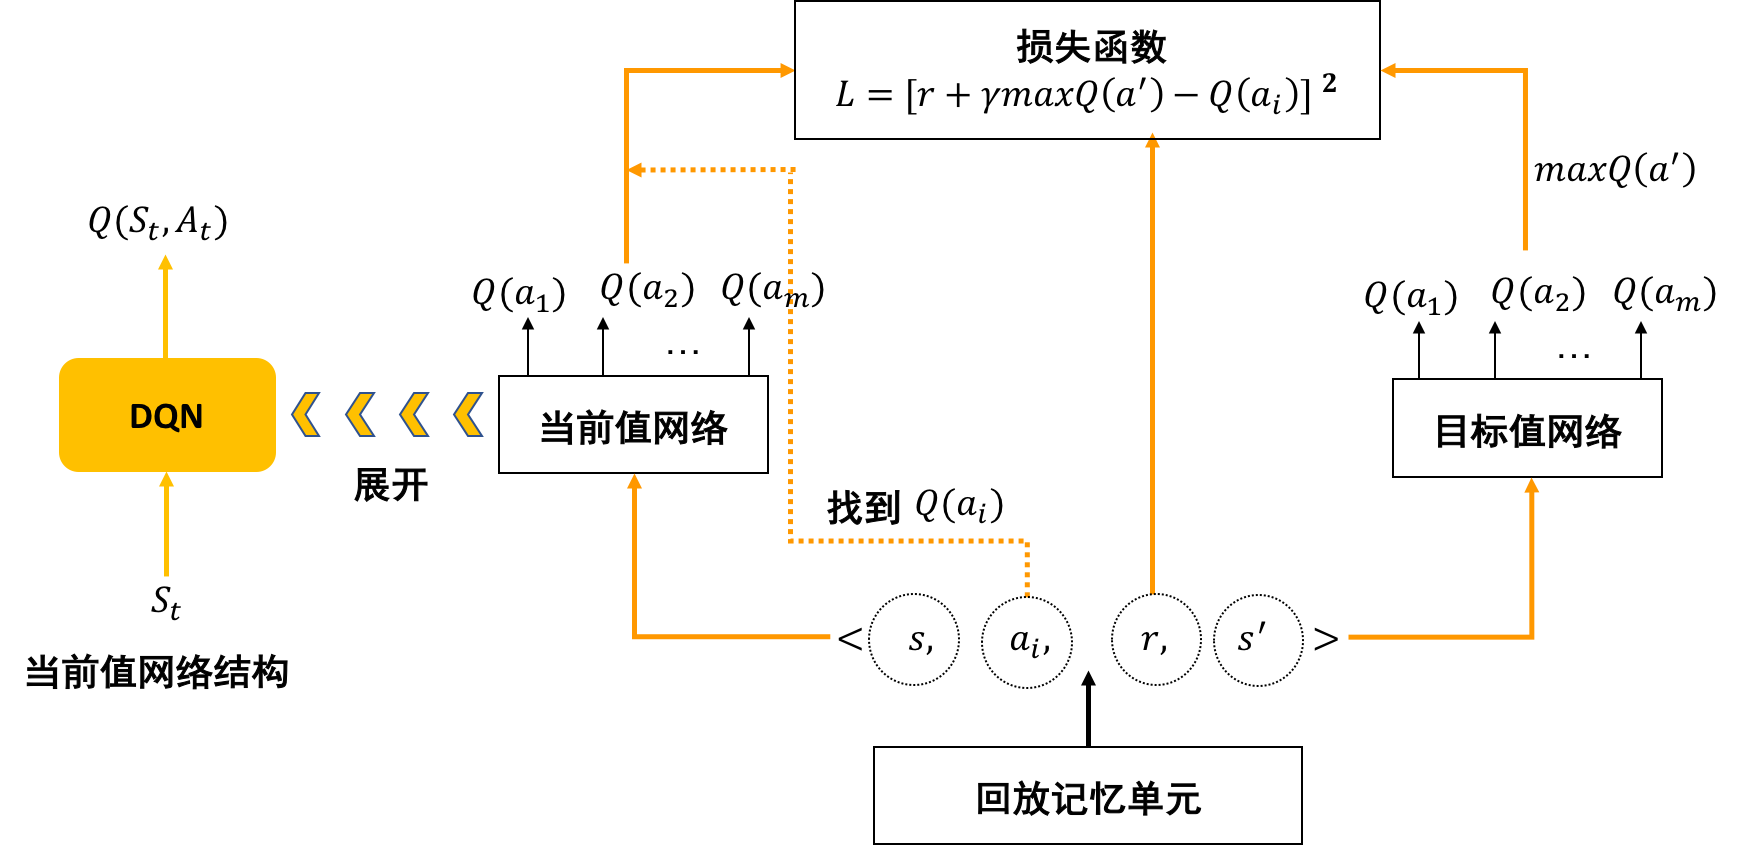
\includegraphics[width=0.9\textwidth]{loss_DQN}
\caption{DQN模型的损失函数构造过程}
\label{fig:loss_DQN}
\end{figure}

\paragraph{DQN基准模型}
可以将DQN模型进行简单的改进后,用于直复营销的策略学习中。在直复营销场景中,不需要在线获取样本来构建回放记忆单元,而可以将提前搜集好的数据进行简单的处理,形成转移样本$<s, a, r, s^{'}>$的格式后,直接进行模型的训练。在本章中,因为主要研究部分可观测的问题,所以为了方便表示,将转移样本表示成$<x, a, r, x
^{'}>$的形式,其中$x$表示客户的观测状态值,$a$表示营销人员所采取的不同营销方式,$r$表示客户所产生的利润(即时奖赏)。修改后的DQN模型的训练过程如算法$\ref{algo:algorithm_DQN}$所示。

从$\ref{algo:algorithm_DQN}$可以看出,在每一轮的迭代中,首先从转移样本集中抽取批数据$\{<X_{t}, A_{t}, R_{t}, X_{t+1}>\}_{t=1,\cdots,B}$,然后当前值网络和目标值网络的输出值,并利用随机梯度下降法更新当前值网络的参数。最后,没经过C步,进行一次参数拷贝,将当前值网络的参数拷贝给目标值网络。当每一轮迭代完毕后,利用测试集测试,具体做法是,将客户的观测值$X_{t}$带入Q当前值网络,并以贪婪的方式从当前值网络中选择最佳的营销行为$\argmax_{a}Q(X_{t},a)$。

\begin{algorithm}[htbp]
 \small
 \SetAlgoLined
 \SetKwRepeat{Repeat}{repeat}{until}
 \KwData{折扣因子$\gamma$,最大迭代轮数$P$,批大小为$B$,学习率为$\alpha$,参数拷贝步数:C,转移样本集$D=\{<X_{j}, A_{j}, R_{j}, X_{j+1}>|j=1,\cdots,N\}$,($N$为转移样本的个数)} 
 \KwResult{输出当前值网络:$\bm{\theta}$}

 使用随机参数$\bm{\theta}$初始化Q值函数(当前值网络)\;
 初始化Q目标值网络$\bm{\theta}^{-}$,令$\bm{\theta}^{-}=\bm{\theta}$\;
 \For((进行每轮迭代)){$epoch=1,\cdots, P$}{
  \For((从转移样本集中随机取批数据)){mini-batch k}{

    批数据为:$\{<X_{j}, A_{j}, R_{j}, X_{j+1}>\}_{j=1}^{B}$\;
    利用Q当前值网络$\bm{\theta}$计算Q估计值:$Q(X_{j}, A_{j};\bm{\theta}^{-})$\;
    利用Q目标值网络$\bm{\theta}^{-}$计算Q目标值:\\
     $\quad$ $R_{j}+\gamma \max_{a^{'}}Q(X_{j+1},a^{'};\bm{\theta}^{-})$\;
    使用随机梯度下降法更新当前网络参数:
    $\bm{\theta}_{t+1}=\bm{\theta}_{t}+\alpha[R_{j}+\gamma \max_{a^{'}}Q(X_{j+1},a^{'};\bm{\theta}^{-})-Q(X_{j}, A_{j};\bm{\theta}^{-})]\triangledown Q(X_{j}, A_{j};\bm{\theta})$\;
    每隔$C$步更新一次Q目标值网络参数,即:$\bm{\theta}^{-}=\bm{\theta}$\;
    }
    利用测试集,测试当前的Q值函数;
 }
 \caption{基于DQN的直复营销模型}
 \label{algo:algorithm_DQN}
 \end{algorithm}

% 图$\ref{fig:dqn_crm}$为DQN当前值网络简化的网络示意图。其中,$O_{t}$为募捐者的观测值,$Q(S_{t},A_{t})$为在$t$时刻时,执行行为$A_{t}$所的到的Q估计值。需要注意的是,在使用DQN模型进行训练时,前一个输入和后一个输入之间是没有关系的。
% \begin{figure}[htbp]
% \centering
% 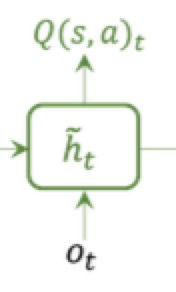
\includegraphics[width=0.2\textwidth]{dqn_crm}
% \caption{DQN当前值网络结构}
% \label{fig:dqn_crm}
% \end{figure}

\subsection{基于RNN的DQN模型}
在将DQN模型应用到Atari游戏中时\citep{mnih2013playing},DeepMind团队之所以会选择卷积神经网络CNN去训练Q值函数,是因为在CNN结构中,通过卷积操作和池化操作可以大幅度的降低网络参数,从而加快神经网络的训练。此外,更重要的是,由于CNN网络的这种特殊训练方法使其非常善于抽取位置不变的特征,特别适合处理图像这类网格型结构的数据,因此广泛应用在图像识别领域。因为视频游戏的输入是也是图像,所以在Atari游戏中,使用CNN结构的神经网络逼近值函数的效果就会很好。

但是,在CNN网络中,假设输入是一个独立的没有上下文联系的单元,即前一个输出和后一个输入是没有关系的,所以CNN网络无法对时间序列上的变化进行建模。而样本出现的时间顺序对于自然语言处理、语音识别、手写体识别等应用非常重要。为了适应这种需求,就出现了另一种神经网络结构——循环神经网络(Recuurent Neural Network, RNN)

 \paragraph{RNN网络}
RNN是一种对序列数据建模的神经网络,可以连接先前的信息到当前的任务上来。具体的做法是:RNN网络会对序列中先前的信息进行记忆存储,并将其应用到当前输出的计算中去,即隐藏层之间的节点不再是无连接的而是有连接的,并且隐藏层的输入不仅包括输入层的输入还包括上一时刻隐藏层的输出。图$\ref{fig:rnn1}$是一个RNN模型的简化结构展开图。
\begin{figure}[htbp]
\centering
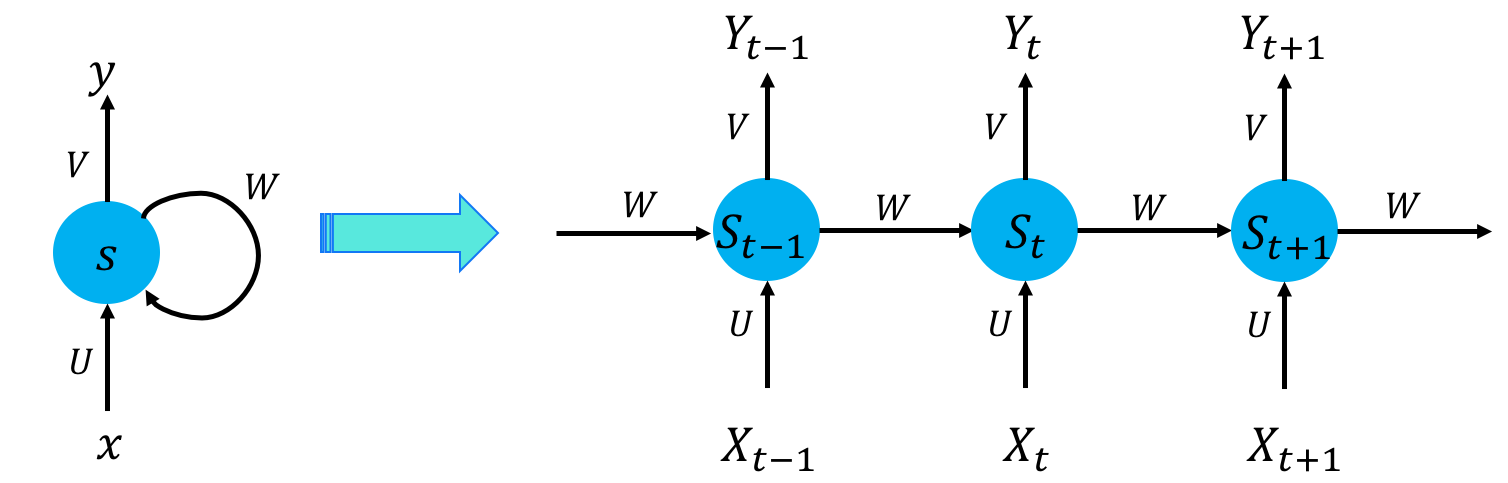
\includegraphics[width=0.8\textwidth]{rnn1}
\caption{RNN网络的简化结构展开图}
\label{fig:rnn1}
\end{figure}

在图$\ref{fig:rnn1}$中,$X_{t}$表示$t$时刻的输入,$S_{t}$表示$t$时刻的隐藏层的记忆值(Memory),记为隐状态,它基于上一时刻的隐状态$S_{t-1}$和当前输入$X_{t}$而得到,
% \begin{equation}
% \begin{aligned}
% s_t=f(U x_{t}+W s_{t-1})
% \end{aligned}
% \end{equation}
% 其中,$f(\cdot)$一般是非线性的激活函数;
% 在计算$s_{0}$时,即第一个单词的隐藏层状态,需要用到$s_{−1}$,但是其并不存在,在实现中一般置为0。
$Y_{t}$表示$t$时刻的输出。另外,$U$是输入层到隐藏层的权重矩阵,$V$是隐藏层到输出层的权重矩阵,$W$是隐藏层上一次的值作为这一次输入的权重矩阵,需要注意的是:在传统神经网络中,每一个网络层的参数是不共享的,而在RNN中,所有层次均共享同样的参数,因此大大地降低了网络中需要学习参数的数量,这反应出在RNN中,每一步操作都是在做相同的工作,只是输入不同。综上,RNN网络在$t$时刻接收到输入$X_{t}$以及上一时刻隐藏层的输出$S_{t-1}$后,可产生新的隐藏层信息$S_{t}$以及输出值$Y_{t}$。
% 特别的,$o_{t}$的值不仅仅取决于$x_{t}$,还取决于$o_{t-1}$。
可以用公式\eqref{rnn_2}和\eqref{rnn_1}来表示循环神经网络的计算方法:
\begin{equation}
\label{rnn_2}
\begin{aligned}
S_{t}=f(U \cdot X_{t}+W \cdot S_{t-1})
\end{aligned}
\end{equation}
\begin{equation}
\label{rnn_1}
\begin{aligned}
Y_{t}=g(V \cdot  S_{t})
\end{aligned}
\end{equation}

其中,式\eqref{rnn_2}是隐藏层的计算公式,它是循环层,$f$是激活函数。式\eqref{rnn_1}是输出层的计算公式,输出层是一个全连接层,也就是说它的每个节点都和隐藏层的每个节点相连,$g$是激活函数。从上面的公式我们可以看出,循环层和全连接层的区别就是循环层多了一个权重矩阵$W$。如果反复把式$\eqref{rnn_2}$带入到式$\eqref{rnn_1}$,可以得到式\eqref{rnn_3}:
\begin{equation}
\label{rnn_3}
\begin{aligned}
Y_{t}&=g(V S_{t})\\
&=V f(U X_{t}+W S_{t-1})\\
&=V f(U X_{t}+W f(U X_{t-1}+W S_{t-2}))\\
&=V f(U X_{t}+W f(U X_{t-1}+W f(U X_{t-2}+W f(U X_{t-3}+\cdots)))\\
\end{aligned}
\end{equation}

从式\eqref{rnn_3}可以看出,循环神经网络RNN的输出值$Y_{t}$,是受前面历次输入值$X_{t}$、$X_{t-1}$、$X_{t-2}$、$X_{t-3}$、$\cdots$影响的,这就是为什么循环神经网络可以往前看任意多个输入值的原因,也是它为什么善于对样本单元按序列进行建模的原因。

RNN网络的训练方法采用了基于时间的反向传播算法(BackPropagation Through Time, BPTT),因为篇幅限制,在此不表,详情参考文献\citep{bersini1997simplification}。
% 但是,在处理较长序列的时候, RNN不能得到较好的性能。一个主要原因是,RNN在训练中如果向前考虑的很远的时候,会导致对应的误差项的值增长或者缩小的非常快,就会很容易发生梯度爆照或者梯度消失的现象,这导致训练时梯度不能在较长序列中一直传递下去,从而使RNN无法捕捉到长时间距离的信息。由此,提出了长短时记忆网络(Long  Short-Term Memory,LSTM)。

% 因为原始RNN的隐藏层只有一个状态,它对于短期的输入非常敏感,LSTM在此基础上增加了一个状态,让它保存长期的状态,从而解决了传统RNN无法处理长距离依赖的问题。新增加的状态称为单元状态(Cell State)。因为篇幅的限制,关于LSTM的原理在此不表,详见文献\citep{hochreiter1997long}。
 \paragraph{DQN_RNN}
 因为RNN网络在时序变化问题中的强大建模能力,所以,为了更好的将强化学习应用在序列相关的问题中,就出现了基于RNN网络的DQN模型\citep{hausknecht2015deep,narasimhan2015language}。在这些研究中,作者普遍采用的做法是,将DQN模型中的CNN网络替换成了RNN网络,希望通过对序列中存在相关性的信息进行建模,来获取更可靠的隐状态信息,进而达到更好的值函数逼近效果。经过实验发现,在文本、语音等序列相关问题上确实取得了比传统基于CNN网络的DQN模型更好的表现\citep{bakker2002reinforcement,hausknecht2015deep,lin1993reinforcement,narasimhan2015language}。

 同样地,在直复营销场景中,客户和营销人员的交互也是一个随时间而不断发生变化的过程。因此,如果使用基于RNN的DQN模型(记作DQN_RNN)对直复营销场景进行建模,将客户的观测信息作为RNN网络的输入,就可以利用RNN网络在序列问题的建模优势,更好的学习客户的隐状态信息,然后再将隐藏层产生的隐状态信息作为客户的真实状态,输入到DQN网络中逼近Q值函数,以进行更好的策略学习。就是通过这种自动获取隐状态的方式,可以在一定程度上解决客户状态的部分可观测问题。

  \begin{figure}[htbp]
 \centering
 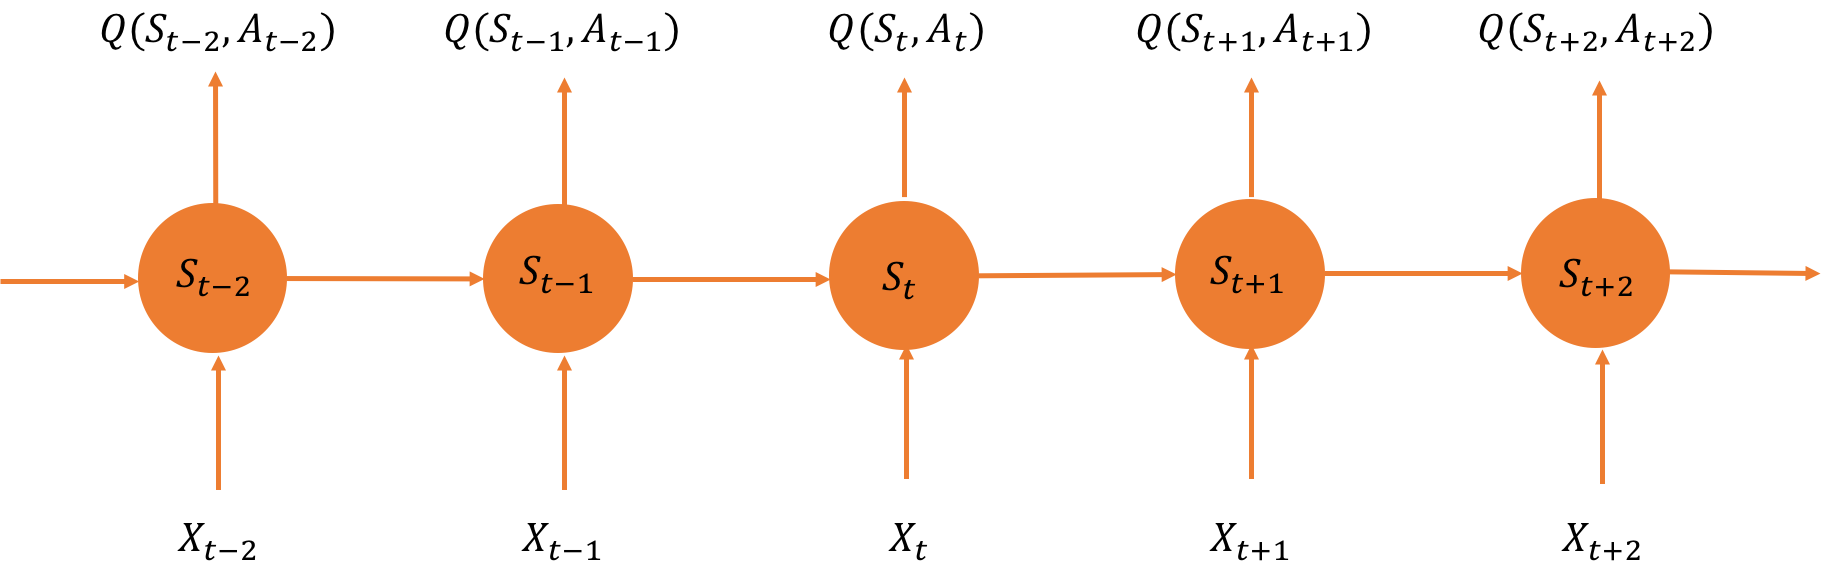
\includegraphics[width=0.9\textwidth]{dqn_rnn1}
 \caption{DQN_RNN当前值网络结构}
 \label{fig:dqn_rnn_1}
 \end{figure}

 参考文献\citep{hausknecht2015deep,narasimhan2015language}所设计的模型,并且结合RNN的结构展开示意图$\ref{fig:rnn1}$,可以得到DQN_RNN模型当前值网络结构的简化示意图$\ref{fig:dqn_rnn_1}$。对应到直复营销场景中,$X_{t}$表示$t$时刻客户的观测信息,$S_{t}$表示$t$时刻RNN学习到的(客户)隐状态信息,$Q(S_{t}, A_{t})$表示在$t$时刻,当隐状态为$S_{t}$且营销人员采取行为$A_{t}$时的Q估计值。因为隐状态$S_{t}$是关于上一时刻隐状态$S_{t-1}$和当前观测值$X_{t}$的函数,所以,Q值网络也是关于当前观测$X_{t}$和上一时刻隐状态$S_{t-1}$的函数。

 与DQN算法$\ref{algo:algorithm_DQN}$相比,DQN\_RNN算法的当前值网络和目标值网络均变成了RNN网络,样本集合中不再是独立的状态转移样本,而是有固定步长$T$的序列$\{<X_{1}, A_{1}, R_{1}, X_{2}, \cdots, X_{T-1}, A_{T-1}, R_{T-1},X_{T}>\}$。所以,从样本集合中抽取批数据进行训练时,也是以序列的形式进行抽取,其他部分与$\ref{algo:algorithm_DQN}$相同。同样地,在损失函数的构造上,DQN\_RNN模型的输入也是有固定步长$T$的序列$\{<X_{1}, A_{1}, R_{1}, X_{2}, \cdots, X_{T-1}, A_{T-1}, R_{T-1},X_{T}>\}$,并且其误差训练方法是按照BPTT的方式进行的\citep{bersini1997simplification},除此之外和DQN模型的损失函数构造过程$\ref{fig:loss_DQN}$相同。


\section{基于RNN的深度强化学习混合模型}
在上述DQN\_RNN的模型中,利用RNN网络的循环结构,本文希望可以在时间变化的序列问题上更好的捕捉到客户状态的隐藏信息(即隐状态),进而更好的逼近Q值函数。所以,在RNN网络的优化过程中同时肩负着两个任务:

\begin{itemize}
\item 序列中关于隐状态表示方法的学习,对应公式\eqref{rnn_2}
\item Q值函数的逼近(最优策略的学习),对应公式\eqref{rnn_1}。
\end{itemize}

% $\\$

% (1)序列中关于隐状态表示方法的学习,对应公式\eqref{rnn_2}。

% (2)Q值函数的逼近(最优策略的学习),对应公式\eqref{rnn_1}。

% $\\$

也就是说,在RNN网络的优化过程中,需要利用目标值网络和当前值网络输出值的均方误差同时进行Q值函数的逼近和隐状态的学习。但是,从该损失函数$L=[r+\gamma \max_{a^{'}}Q(s^{'},a^{'};\bm{\theta}^{-})-Q(s,a;\bm{\theta})]^{2}$)的构造上看,其在更新的过程中更强调对Q值函数误差的学习,而没有专门对隐状态所产生的误差进行学习。所以本文认为,DQN\_RNN这种网络结构不能很好的学习隐状态的表示方法,即不能很好的处理强化学习中的部分可观测问题,进而也就会影响到最优值函数的学习。

针对DQN\_RNN模型存在的以上问题,本节提出了基于两个神经网络的强化学习混合模型。另外,根据训练方式的不同,又分为RNN+DQN$^{*}$双网络独立训练模型、1-RNN+DQN一步联合训练混合模型和2-RNN+DQN两步联合训练混合模型。特别要强调的是,因为本章的应用场景并不涉及图像,所以为了方便试验进行,本节中DQN模型的值网络均使用深度神经网络(Deep Neural Networks, DNN)来代替。

\subsection{双网络独立训练模型}
如上文所述,对于只有一个RNN网络的DQN\_RNN模型来说,在网络优化的过程中,同时兼具序列隐状态的学习和近似最优策略的学习是比较困难的。那么,一个很自然的想法是,可以使用两个网络对以上这两个任务分别进行有针对性的学习,由此便得到双网络独立训练模型。具体地,使用RNN网络单独对序列中的隐状态表示方法进行学习,使用DQN网络对Q值函数进行逼近,以学到更好的值函数,本文将此模型记作:RNN+DQN$^{*}$。

RNN+DQN$^{*}$模型的网络结构如图$\ref{fig:rnn+dqn}$所示,共包括两个网络。其中,蓝色部分为RNN网络,图中$X_{t}$表示$t$时刻的观测值,$S_{t}$表示$t$时刻的隐状态信息,$R(S_{t}, A_{t})$表示$t+1$时刻预测的奖赏值。
% ,$R_{t}^{'}$为预测的奖赏值。
黄色部分为DQN网络,其中,$Q(S_{t},A_{t})$是$t$时刻Q的估计值。
\begin{figure}[htbp]
\centering
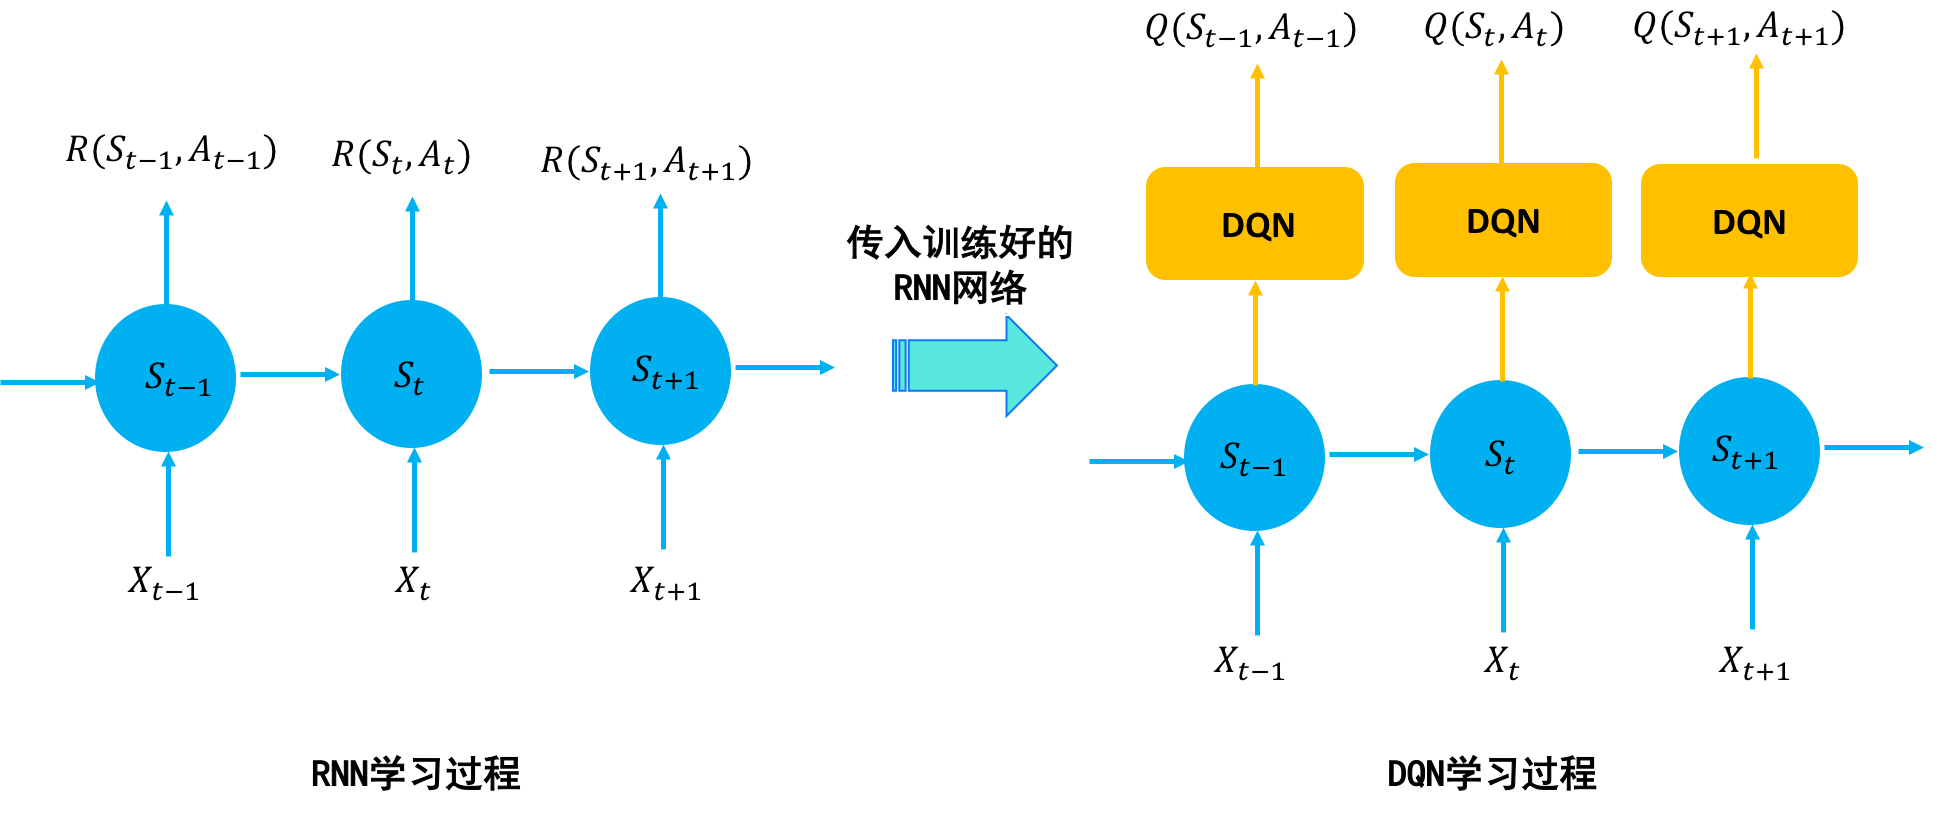
\includegraphics[width=1.0\textwidth]{rnn+dqn_}
\caption{RNN+DQN$^{*}$模型的网络结构}
\label{fig:rnn+dqn}
\end{figure}

从图$\ref{fig:rnn+dqn}$可以看出RNN+DQN$^{*}$模型的学习过程也包括两个部分,具体可概括为:

(1)首先,进行RNN网络的训练:利用循环神经网络RNN对交互序列$\{<X_{1}, A_{1}, R_{1}, X_{2}, \cdots, X_{T-1}, A_{T-1}, R_{T-1},X_{T}>\}$中的观测值$X_{t}$、奖赏值$R_{t}$和行为$A_{t}$等监督数据进行学习(通过观测值预测不同行为下的奖赏值),通过捕捉监督数据中的序列相关性,以学习到更好的隐状态表示方法。

(2)待RNN网络训练完毕后,进入DQN网络的训练:将观测值$X_{t}$和上一时刻的隐状态信息$S_{t-1}$输入到学好的RNN网络后,RNN网络会输出其对应的隐状态$S_{t}$,然后再将该隐状态信息$S_{t}$作为强化学习中的状态输入到DQN网络中,最后依靠DQN网络强大的非线性表达能力逼近Q值函数,进行更高效的策略学习,以达到最大化累积奖赏的目的。

显然,第一部分属于监督学习过程,利用监督数据充分发挥RNN网络对时间序列建模的优势,以更好的学习隐状态信息;第二部分属于强化学习过程,通过DQN的参数更新方法以及DNN网络的非线性逼近能力,可以更好的进行值函数的学习。按照这种方法,可以让这两个网络的实现优势互补,以在实际应用中更好的解决状态的部分可观测问题,进而产生更高效的策略。

在RNN+DQN$^{*}$模型的测试阶段,将上一时刻的隐状态信息和这一时刻的观测值输入到RNN网络中,然后再将产生的新隐状态信息输入到已经学习好的Q值网络中,最后以贪婪的方式选择最优的行为。

同样,RNN+DQN$^{*}$模型的误差构造过程也分为两个部分,如图$\ref{fig:dqn_rnn_loss}$所示。左边为RNN监督学习的误差构造过程,主要是利用观测值$x$来预测行为$a_{i}$下的奖赏值$r(a_{i})$,然后使用预测的奖赏值$r(a_{i})$和与真实奖赏值$r$之间的误差来构造损失函数进行RNN网络的训练。右边为DQN网络的误差构造过程,虽然和之前DQN网络的误差构造方法相同,都是利用Q目标值和Q估计值的均方误差作为损失函数,但是两个网络的输入变成了由RNN产生的隐状态值。
\begin{figure}[htbp]
\centering
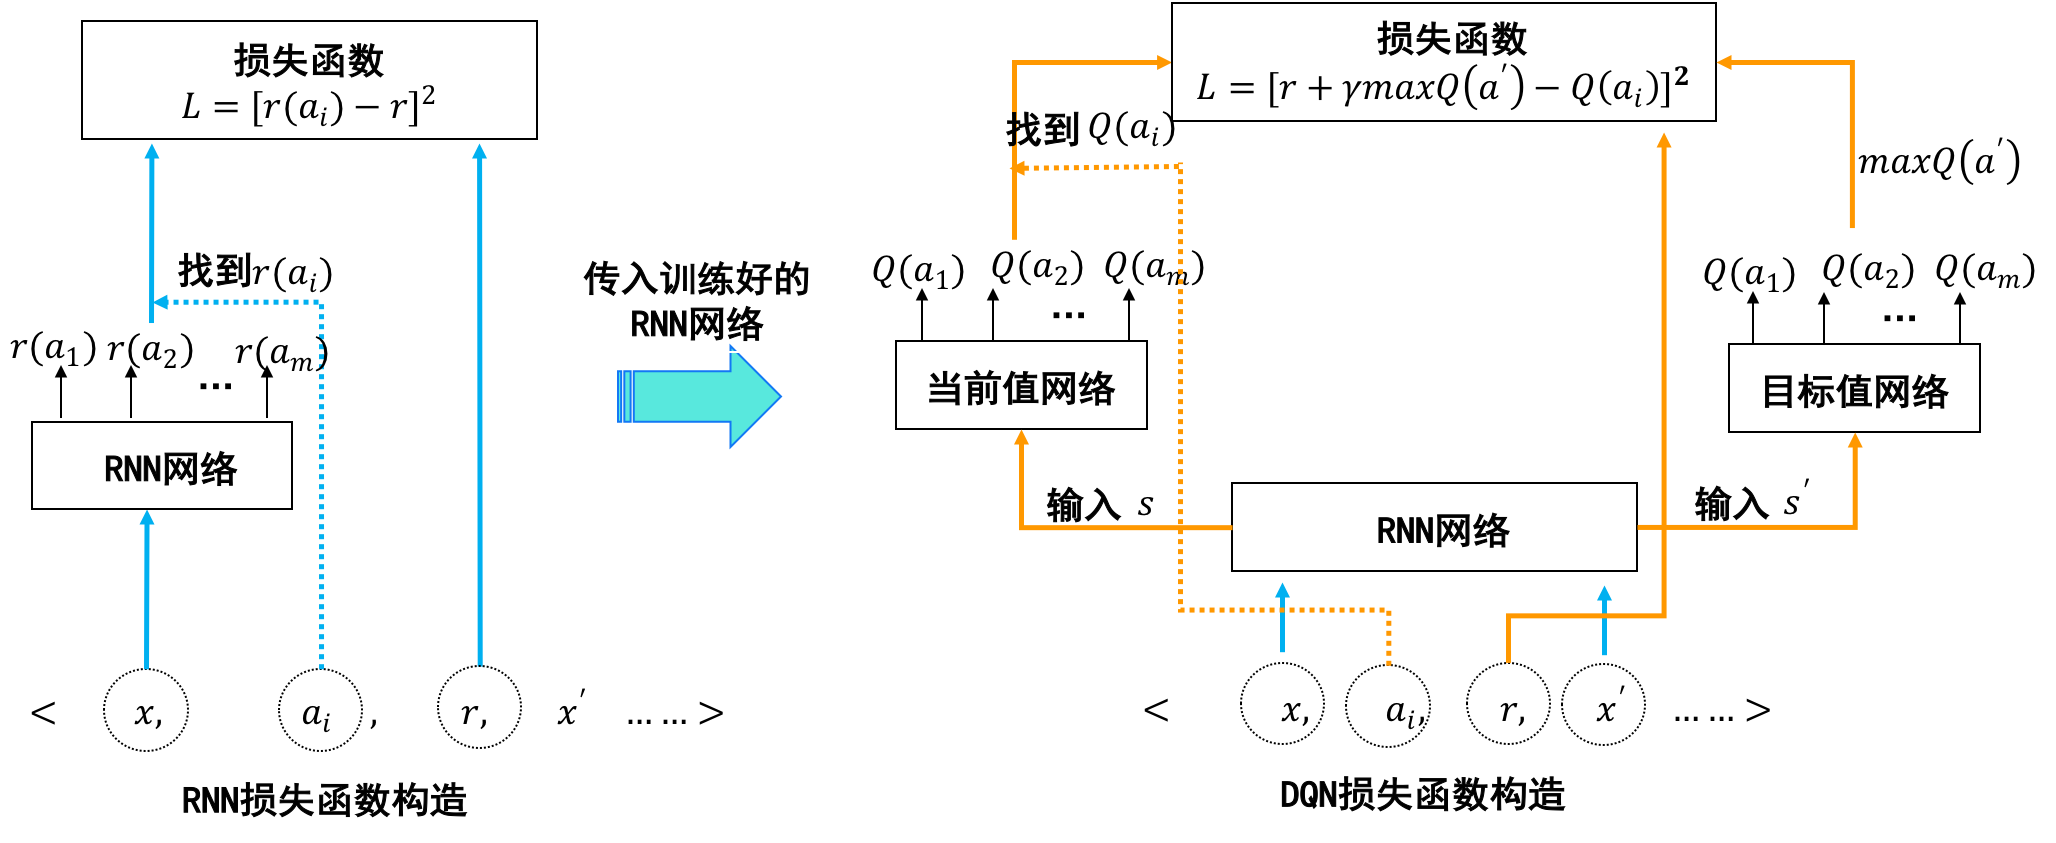
\includegraphics[width=1.0\textwidth]{dqn_rnn_loss}
\caption{RNN+DQN$^{*}$模型损失函数构造过程}
\label{fig:dqn_rnn_loss}
\end{figure}

\subsection{一步联合训练混合模型}
在RNN+DQN$^{*}$模型中,虽然充分利用了RNN网络和DQN网络各自的优点,但是,两个网络的训练过程被完全割裂开了,这样就会造成的一个问题:很难知道已经训练好的RNN网络是否有能力可以让DQN网络学到最优的Q值函数,或者说很难知道RNN网络训练到什么程度才可以让DQN更好的产生一个Q值函数。基于这个想法,提出一种可以让RNN网络和DQN网络联合进行训练的模型,记为1-RNN+DQN模型

1-RNN+DQN的网络结构如图$\ref{fig:1_dqn_rnn}$所示,其中,$X_{t}$是$t$时刻的观测值,$S_{t}$是$t$时刻的隐状态信息,$R(S_{t},A_{t})$是在$t$时刻预测的奖赏值。$Q(S_{t},A_{t})$表示$t$时刻预测的Q值。蓝色部分对应着RNN网络的监督学习部分,黄色部分对应着DQN的强化学习部分。
\begin{figure}[htbp]
\centering
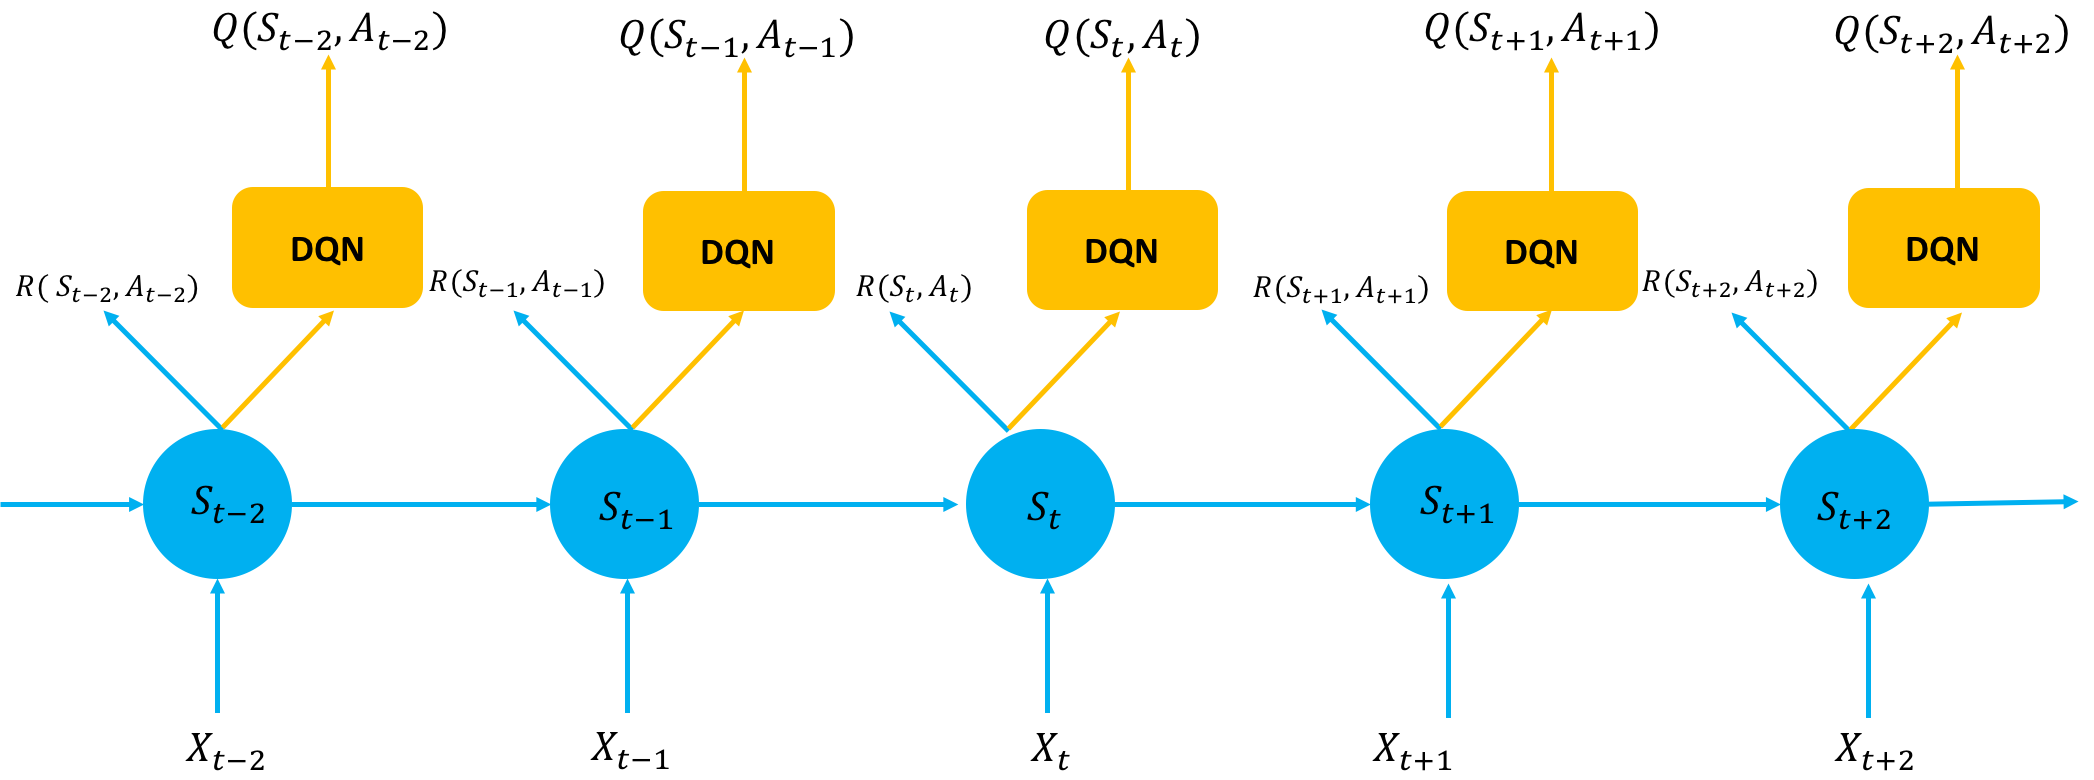
\includegraphics[width=1.0\textwidth]{1_dqn_rnn}
\caption{1-RNN+DQN模型网络结构}
\label{fig:1_dqn_rnn}
\end{figure}

从图$\ref{fig:1_dqn_rnn}$中可以看出,在1-RNN+DQN模型的学习过程中,RNN网络在交互序列$\{<X_{1}, A_{1}, R_{1}, X_{2}, \cdots, X_{T-1}, A_{T-1}, R_{T-1},X_{T}>\}$的每一时间步上进行一次隐状态的更新后,就在下一时刻将由此隐状态和下一时刻的输入所产生的新的隐状态作为了DQN模型的输入状态。具体地,在$t-1$时刻,利用监督信号(观测值$X_{t-1}$和奖赏$R_{t-1}$)来更新RNN网络,并将此时刻产生的隐状态$S_{t-1}$传入到下一时刻,在$t$时刻,将观测值$X_{t}$和隐状态$S_{t-1}$带入到公式\eqref{rnn_2}中,计算出$t$时刻新的隐状态$S_{t}$,然后再将此隐状态传入到DQN网络,作为强化学习的输入状态,进行DQN网络的更新。两个网络在每一时间步上交替进行更新,直到DQN网络学到一个好的Q值函数,就停止学习。

在测试阶段,与DQN\_RNN模型类似,将观测信息输入RNN网络,然后将RNN网络产生的隐藏信息作为强化学习的输入状态导入到训练好的Q值网络中,以贪恋的方式选择最优行为。


图$\ref{fig:1_dqn_rnn_loss}$为1-RNN+DQN模型的损失函数构造过程。从图$\ref{fig:1_dqn_rnn_loss}$可以看出,其损失函数的构造过程和RNN+DQN$^{*}$模型相似,只是两个网络不再分开进行参数更新,而是同时使用同一交互序列依次交替进行更新。需要指出的是,在训练的过程中,
使用监督信号来进行RNN的隐状态学习,此时需要将监督学习的误差反向传播到RNN网络的头部,但是,DQN网络的误差信号只反向传播到RNN网络的隐藏层,并不参于RNN网络的训练。如所示,1-RNN+DQN模型的误差构造过程和RNN+DQN$^{*}$的误差构造过程类似,只是没有没有分开进行,而是依次交替进行。

因为在1-RNN+DQN模型的学习过程中,RNN网络和DQN网络按照上述训练方法依次进行,学习期间没有发生网络结构的变化,因此称之为一步混合模型。
\begin{figure}[htbp]
\centering
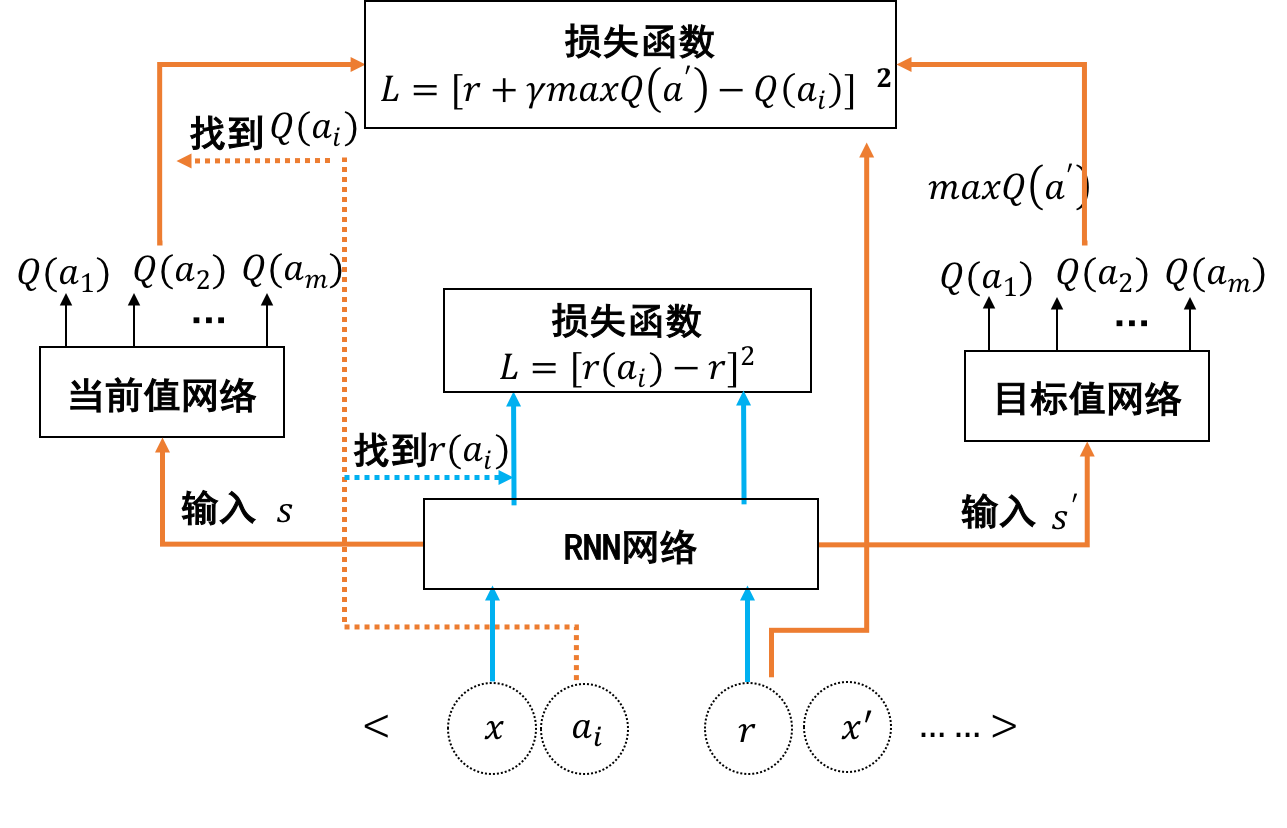
\includegraphics[width=0.8\textwidth]{1_dqn_rnn_loss}
\caption{1-RNN+DQN模型损失函数构造过程}
\label{fig:1_dqn_rnn_loss}
\end{figure}

\subsection{两步联合训练混合模型}
在1-RNN+DQN模型中,通过使用联合训练的方法,可以更容易的为DQN网络的训练找到合适的RNN网络模型,以使得更好的逼近Q值函数。但是,如上文所述:在RNN网络训练的过程中,监督信号的误差传递到了RNN的头部,而在DQN网络的训练过程中,误差信号只传递到RNN的隐藏层,也就是说两个网络之间并没有进行误差的传递。

在1-RNN+DQN模型中,当进行DQN网络的参数更新时,DQN网络是完全信任RNN网络的隐状态表达能力的,所以,其实DQN网络学习的是关于隐状态的一个函数。但是,现实应用的最终的目标是希望模型可以学习到观测值和Q值函数之间的关系,而1-RNN+DQN模型却割裂了Q值函数和观测值之间的直接关系。因此,为了构建Q值和观测值之间直接关系的同时又要保持监督学习学习隐状态的优势,一个想法是:在1-RNN+DQN模型的训练过程中,当进行最后$n$轮(epoch)的训练时,抛弃监督学习的过程,而将Q值的误差信息反向传播到RNN网络的头部,来同时更新RNN网络和DQN网络,进行参数的整体微调,这样就可以将观测值和Q值函数联系到一起了,期望会在一定程度上提升模型的效果。

\begin{figure}[htbp]
\centering
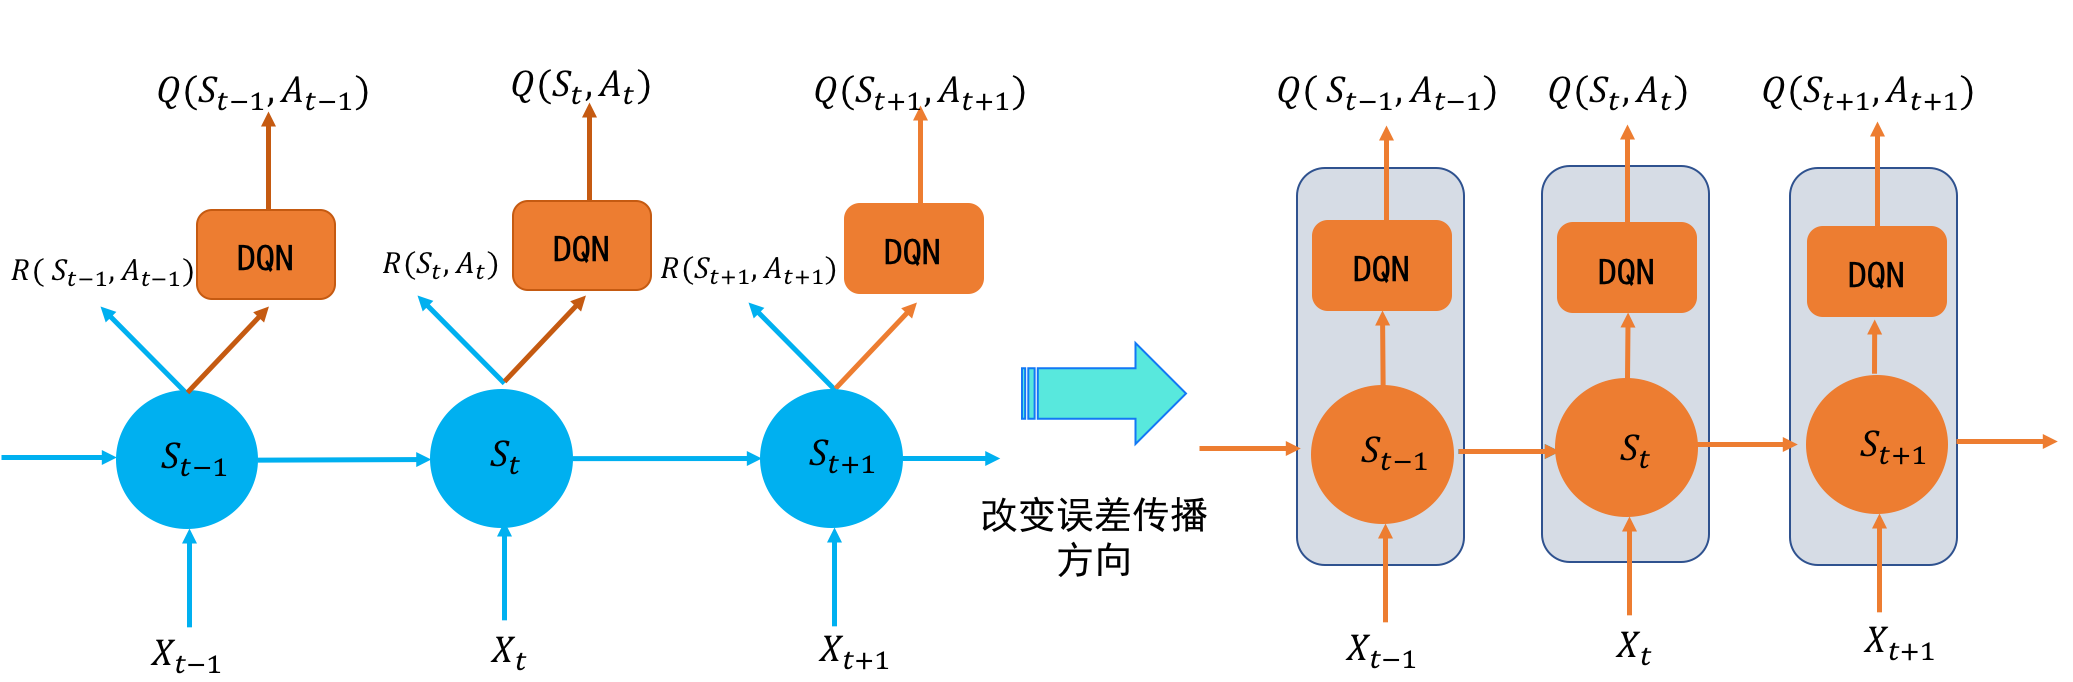
\includegraphics[width=1.0\textwidth]{2_dqn_rnn}
\caption{2-RNN+DQN模型网络结构}
\label{fig:2_dqn_rnn}
\end{figure}

所以,基于以上的想法,本节提出了两步联合训练混合模型,记为2-RNN+DQN。如图$\ref{fig:2_dqn_rnn}$所示,左边为1-RNN+DQN的网络结构,右边是新的网络结构,其中,$X_{t}$是$t$时刻的观测值,$Q(S_{t},A_{t})$表示在t时刻预测的Q值函数。从图$\ref{fig:2_dqn_rnn}$中可以看出,2-RNN+DQN模型在训练时共分为两个阶段,第一阶段,按照1-RNN+DQN的方法进行训练,学习到两个网络的参数向量$\bm{\theta}^{'}$和$\bm{\theta}^{''}$;第二阶段,将RNN网络的隐藏层和DQN网络的输入层连接起来,组成一个新的网络结构$[\bm{\theta}^{'},\bm{\theta}^{''}]$,新的网络的输入是观测值$X_{t}$,输出是Q函数。图$\ref{fig:2_dqn_rnn_loss}$为第二阶段的损失函数构建过程,从图中可以看到,当前值网络和目标值网络所构成的损失函数的误差直接传播到了RNN的输入层,也就是状态的观测值,然后再同时进行两个网络的参数更新。

在测试阶段,将观测值输入到第二阶段新的网络结构中,通过贪婪的方式从Q值函数中选择最佳的行为。

% 训练时两个阶段训练时间应该如何把握。本实验采用的方法是将训练数据集按照8:2的比例分成两份,第一份用于第一阶段的训练,第二份用于第二阶段的训练。

\begin{figure}[htbp]
\centering
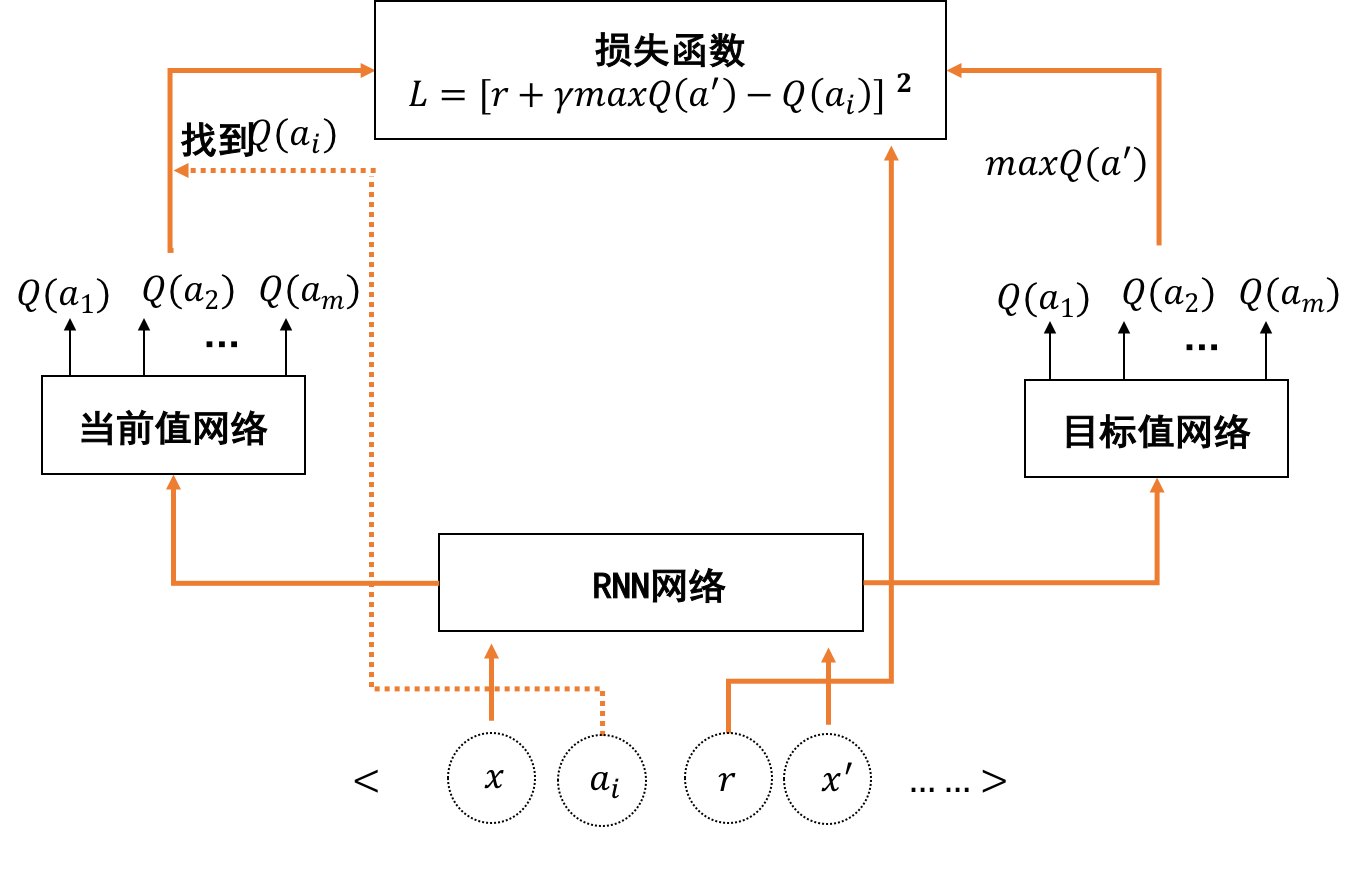
\includegraphics[width=0.8\textwidth]{2_dqn_rnn_loss}
\caption{2-RNN+DQN模型损失函数构造过程}
\label{fig:2_dqn_rnn_loss}
\end{figure}

\section{实验仿真}
在本节中,首先对所使用的数据进行说明,然后阐述仿真环境的构建方法,接着介绍本章试验所用的模型以及试验设置信息,最后从模型的长期收益、不同数据收集方式下所产生的收益、不同数据规模下所产生的收益等三方面对模型的结果进行对比,并分析。

\subsection{数据集}
本章试验仍然选择使用UCI数据库中关于直邮营销著名的公开数据集KDD-CUP 1998\footnote{https://kdd.ics.uci.edu/databases/kddcup98/kddcup98.html}作为模型训练、测试以及构建仿真环境的数据集。但是,因为本文没有考虑可变时间的因素,所以,为了减少可变时间间隔给模型训练带来的影响,从数据库中取出了间隔较大的8组营销数据,只保留了营销编号从4到18的数据,所以每个募捐者的交互序列上只有15个时间步的交互序列,可表示为:$<X_{1},A_{1},R_{1},\cdots,X_{14},A_{14},R_{14},X_{15}>$。除此之外,在用户特征和营销行为的选择上,和第三章也有所不同,具体如下:

% 将原始数据集中每个募捐者的交互序列看成一个含有23个时间步的交互序列,,当涉及RNN网络的训练时,其输入是如上所示的交互序列,当涉及DNN的训练时,需要将交互序列分割成单独的转移样本$\{<X_{t},A_{t},R_{t},X_{t+1}>\}_{t=1,2,\cdots}$的形式。其中,

(1)$X_{t}$:表示每个募捐者在$t$时刻的观测特征值,本节所使用的用户观测特征是从第三章表~\ref{tab:obser_donors}中抽取的五维数据所组成的向量,如表~\ref{tab:obser_donors4}所示,这些特征的计算方法和第三章中使用的方法相同:
\begin{table}[htbp]
  \centering
  \caption{捐助者观测特征的选取}
  \label{tab:obser_donors4}
  \begin{tabular}{ll}
    \toprule
      特征 & 描述 \\
    \midrule
      % age & 捐助者的年龄 \\
      % income & 捐助者的收入 \\
      ngiftall & 捐助者的捐助的次数 \\
      numprom & 向该捐者发送邮件的次数 \\
      frequency & 该捐助者捐助的频率:numgiftall/numprom\\
      ramntall & 捐助的总金额 \\
      recency & 距离上一次捐助的时间 \\
      % nrecproms & 之前六个月里,给该捐者者发送直邮营销的次数\\
      % nrecgifts & 之前六个月里,捐助者捐助的次数\\          	  
    \bottomrule
  \end{tabular}
\end{table}

(2)$A_{t}$:表示营销人员在$t$时刻所采取的营销行为。需要特别注意的是,为了增加行为的多样性,本节的行为选取和第三章也不同,在KDD-CUP 1998的数据集中,可以找到11种不同类型的邮件(代号分别为:LL,WL,CC,FS,NK,SK,TK,GK,XK,X1,G1),再加上不发送邮件这一营销行为,因此本节的行为集合中一共有12个行为。所以,本节模型学习的策略就变成了:PVA应该给不同的捐助者发送什么类型的邮件,可以使的所获得的长期收益最大化,而不仅仅是选择发送或者不发送。

(3)$R_{t}$:表示营销人员在$t$时刻执行营销行为所带来的奖赏,和第三章一样,本节使用PVA从捐助者那里获得的利润作为对应的奖赏信息。

\subsection{仿真环境}
\paragraph{仿真环境构造}
本章所构造的仿真环境和第三章仿真环境的构造过程大致相同。都需要构造两个模型:捐助者的响应概率的模型$P(s,a)$和即时奖赏模型$A(s,a)$。但是不同的是,本节实验中,两个模型均采用RNN网络来进行建模,期望借助RNN网络在序列问题上的建模优势来获得更准确的响应模型和即时奖赏的预测模型。

具体地,使用$P(s,a)$模型预测$t$时刻捐助者的状态转移概率时,是使用$t$时刻时捐助者的隐状态$S_{t}$来进行预测的,也就是说模型$P(s,a)$是关于观测值$X_{t}$和上一时刻隐状态$S_{t-1}$的函数。同样,$A(s,a)$模型也与之相同。网络结构可表示为图$\ref{fig:rnn_q_p}$。

\begin{figure}[htbp]
\centering
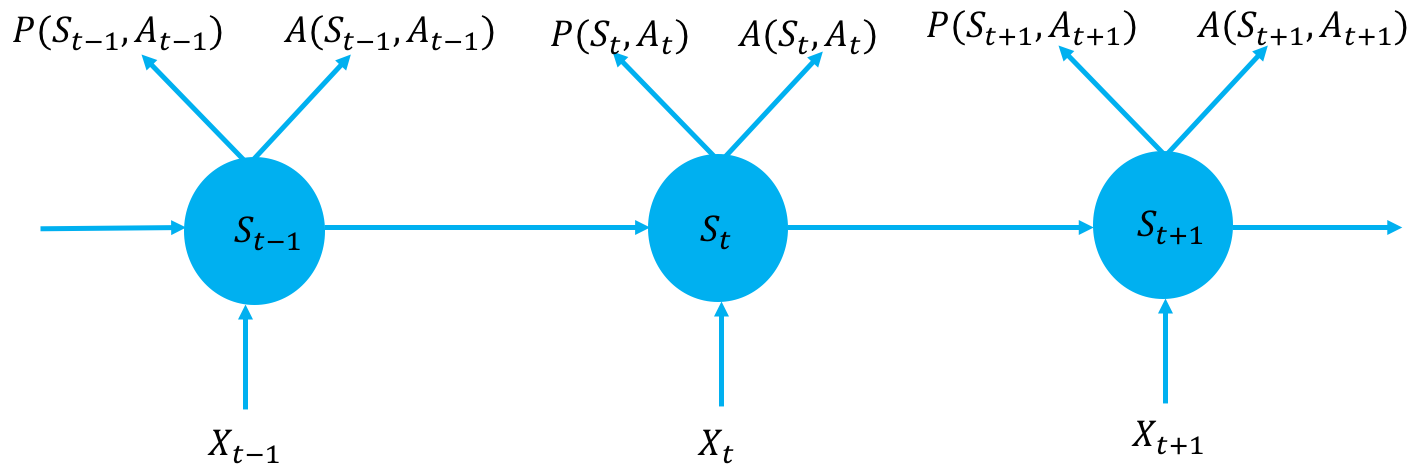
\includegraphics[width=0.8\textwidth]{rnn_q_p}
\caption{模型P(s,a)和模型A(s,a)的网络结构}
\label{fig:rnn_q_p}
\end{figure}

有了模型$P(s,a)$和$A(s,a)$,就可以按照第三章所述方法构建马尔科夫决策过程,参考图$\ref{fig:simulation}$

\paragraph{仿真评估方法}
仿照第三章的评估方法,使用如下方式进行模型的评估:

(1)首先,随机选择一定数量规模的捐助者,并设置他们的初始状态。本实验中将所选择的捐助者的初始状态设置为第4次营销活动时的状态。

(2)然后,使用训练好的强化学习模型输出营销策略:对每个捐助者应该发送哪一种邮件类型。

(3)最后,使用模型$P(s,a)$和$A(s,a)$,得到预估的即时奖赏以及下一时刻的状态。记录这些得到的信息,然后进入下一次的营销决策中。

就这样,按照上述的三个步骤,每循环一次就会模拟一次虚拟的直邮营销的过程。本节实验中,重复循环20次,就得到了20次的模拟营销的效果数据。


\subsection{基准模型和试验设置}
如上文所述,本文所解决的场景不需要处理图像等信息,因此为了简化模型,将DQN中的CNN模型换成深度神经网络DNN,因为DNN网络也是一个无上下文联系的网络,同样可以达到本章所希望比较的效果。

\paragraph{基准模型}
为了比较强化学习和监督学习的在序列决策问题上的优缺点,在本节实验中,分别使用DNN网络和RNN网络来进行营销策略的制定。

在使用DNN网络进行监督学习时,首先需要将捐助者的交互序列分割成转移样本$\{<X_{t},A_{t},R_{t},X_{t+1}>\}_{t=1,2,\cdots}$的形式,然后再使用样本中的($X_{t},A_{t}$)信息来预测即时奖赏$R_{t}$。在测试的时候,将募捐者的观测值作为DNN模型的输入,然后按照贪婪的方式选择选择最优的营销行为:$\argmax_{a} M(o,a)$,其中$M$代表DNN网络学到的模型。

在使用RNN网络进行监督学习时,基于观测值$X_{t}$、上一时刻的隐状态信息$S_{t-1}$以及奖赏信息$R_{t}$来进行RNN网络的更新。在测试时,将募捐者的当前的观测值和上一时刻的隐状态信息带入RNN网络,然后按照贪婪的方式选择最优的营销行为:$\argmax_{a} H(s,a)$,其中$H$代表RNN网络学到的模型。

\paragraph{试验设置}
到目前为止,本实验中提到的模型一共有七个,如表~\ref{tab:4modesl}所示,其中包括两个监督学习模型和5个强化学习模型。
 \begin{table}[htbp]
  \centering
  \caption{本节实验中用到的模型}
  \label{tab:4modesl}
  \begin{tabular}{llp{10cm}}  
    \toprule
      序号 & 模型 & 描述 \\
    \midrule
      1 & DNN & 监督学习\\
      2 & RNN & 监督学习\\
      3 & DQN & 强化学习,使用DNN网络逼近值函数\\
      4 & DQN_RNN & 强化学习,使用RNN网络逼近值函数\\
      5 & RNN+DQN$^{*}$ & 强化学习,使用RNN网络学习隐状态,使用DNN网络逼近值函数,两网络单独训练\\
      6 & 1-RNN+DQN & 强化学习,使用RNN网络学习隐状态,使用DNN网络逼近值函数,两网络联合训练\\
      7 & 2-RNN+DQN & 强化学习,使用RNN网络学习隐状态,使用DNN网络逼近值函数,分两步训练 \\        	  
    \bottomrule
  \end{tabular}
\end{table}

在表~\ref{tab:4modesl}中的七个模型中,一共涉及两个网络RNN和DNN,为了方便比较,所有试验中的RNN网络、  DNN网络以及强化学习(RL)部分参数设置都相同,如表~\ref{tab:4wangluocanshu}所示。

 \begin{table}[htbp]
  \centering
  \caption{参数设置}
  \label{tab:4wangluocanshu}
	% \begin{tabular}{p{0.9\columnwidth}} 
  \begin{tabular}{lp{12.1cm}}  
    \toprule
      模型 & 主要参数描述 \\
    \midrule
      RNN &一个隐藏层。其中:批(batch)大小:32,记忆单元(cell)个数:32 ,学习率:0.003\\
      DNN &两个隐藏层。其中:批(batch)大小:64,第一个隐藏层神经元个数:16 ,第二个隐藏层神经元个数:32,学习率:0.003\\
      RL部分 & 衰减因子:$\gamma=0.88$,每200步进行一次参数拷贝 \\ 
      其它 & 每个模型进行五次试验,每次试验进行30轮(epoch),在每轮训练结束后利用测试集进行模型的测试,将五次试验中每一轮的平均值作为该轮最后的结果值。另外,在2-RNN+DQN模型的训练中,在模型的最后2轮时进行模型的切换(因为经过试验发现,1-RNN+DQN在第20轮就可以收敛。)\\       	  
    \bottomrule
  \end{tabular}
\end{table}

最后,所有模型运行在Mac Pro机器上,内存16GB,试验语言:Python,神经网络基于Tensorflow(版本1.2)编写。

\subsection{仿真结果}
\paragraph{长期收益}

 首先比较以上七个模型在20次模拟直邮中的长期总收益。从原始数据集中抽取20,000个捐助者的交互序列作为模型的训练数据,然后再抽取5000个捐助者的第5次营销的状态作为测试数据。

 在每次试验中,每当进行完一轮的训练后,便将测试数据带入学习好的模型中,按照上述仿真环境中的评估方法进行测试,输出此时模型产生的策略总收益。表~\ref{tab:4result1}展示了七个模型在五次试验中每轮的平均利润值,图[]展示了随着训练时间的不断推移,其中五个强化学习模型产生输出策略的变化情况。

  \begin{table}[htbp]
  \centering
  \footnotesize
  \caption{}
  \label{tab:4result1}
  \begin{tabular}{lllllllllllllllllllllllllllllll}  
    \toprule
      epoch序号 &1&2&3&4&5&6&7&8&9&10\\
    \midrule
      DNN &2222&2222&2222&2222&2222&2222&2222&2222&2222&2222\\
      RNN & \\
      DQN & \\
      DQN_RNN & \\
      RNN+DQN$^{*}$ & \\
      1-RNN+DQN & \\
      2-RNN+DQN & \\
     % \bottomrule
     \toprule
      epoch序号 &11&12&13&14&15&16&17&18&19&20\\
    \midrule
      DNN &2222&2222&2222&2222&2222&2222&2222&2222&22222&2222\\
      RNN & \\
      DQN & \\
      DQN_RNN & \\
      RNN+DQN$^{*}$ & \\
      1-RNN+DQN & \\
      2-RNN+DQN & \\
    % \bottomrule
     \toprule
      epoch序号 &21&22&23&24&25&26&27&28&29&30\\
    \midrule
      DNN &2222&2222&2222&2222&2222&2222&2222&2222&22222&$\bm{2222}$\\
      RNN & \\
      DQN & \\
      DQN_RNN & \\
      RNN+DQN$^{*}$ & \\
      1-RNN+DQN & \\
      2-RNN+DQN & \\
    \bottomrule
  \end{tabular}
\end{table}

从表~\ref{tab:4result1}中第30轮的结果中可以看出,强化学习方法所产生长期利润明显高于监督学习方法所产生的收益,这一点和第三章试验得出结论相同。

从图中可以看出,在使用RNN的强化学习模型DQN_RNN比使用DNN的DQN模型产生的收益要高,而且收敛的速度要快,这主要是因为RNN模型从募捐着的交互序列中捕捉到了时间变化关系。另外,DQN_RNN模型和RNN+DQN$^{*}$模型相比,RNN+DQN$^{*}$模型的产生的收益更多,因为在RNN+DQN$^{*}$模型中,使用监督数据更好的学习到了隐状态的表示方法,给强化学习输入了更准确的状态信息。1-RNN+DQN模型和RNN+DQN$^{*}$模型相比,虽然1-RNN+DQN模型在最初的几轮中的收益没有RNN+DQN$^{*}$多,但是随着试验次数的增加,1-RNN+DQN模型的收益超过了RNN+DQN$^{*}$模型,从而验证了联合训练方法的高效,这是因为在联合训练时,更容易找到合适的RNN模型。2-RNN+DQN在第25轮后发生了模型转换,相比1-RNN+DQN模型产生了更高的收益。

\paragraph{数据收集方式对模型的影响}

 为了考察不同数据收集方式对模型的影响,本部分考虑利用仿真环境重新构建数据集。具体地,随机抽取20,000个捐助者的交互序列数据,然后将他们的初始状态代入到仿真环境中,通过随机的方式从行为集合中选取营销行为,并在仿真环境中执行,得到捐助者的下一状态和此时的奖赏信息,然后将此信息作为捐助者的$t=1$时刻的交互数据,按照这种方式,重复进行15次,就会得到了20,000个捐助者包涵15个时间步的交互序列。

 然后将此数据集带入到上述七个模型中按照第一部分相同的方法进行训练,同样会得到每轮产生的利润,为了减少图标所占空间,此处只展示第30轮各模型所产生的结果,如表~\ref{tab:4result2}所示。将第一部分使用原始数据的结果和使用新构造的数据集所产生的结果绘制成图。

  \begin{table}[htbp]
  \centering
  \footnotesize
  \caption{}
  \label{tab:4result2}
  \begin{tabular}{lccccccccccc}  
     \toprule
      模型 &DNN&RNN&DQN&DQN_RNN&RNN+DQN$^{*}$&1-RNN+DQN&2-RNN+DQN\\
    \midrule
      结果 &2222&2222&2222&2222&2222&2222&2222&\\
    \bottomrule
  \end{tabular}
\end{table}

从图中可以看出,采用随机选取策略的方式得到的收益明显大于按照PVA给定的数据集训练所得的结果。这在一定程度上说明了,PVA的实际数据收集政策似乎是确定性的,同一步骤对所有捐助者采取同样的行动。因此,这个数据集很少或根本没有探索。这说明了正确而充分的探索对于强化学习学习到好的策略时很重要的。

另外,从图中可以看出,RNN和DNN网络输出的结果前后差别并不是很大。这说明了相比监督学习,强化学习受数据收集方式的影响更加敏感,因为强化学习在学习的过程中试图去预测将来会发生什么,探索的越少,对强化学习来说就会引入更多的误差。所以,在实际的应用中,如果要想使用强化学习产生更好的策略,前期在进行数据搜集的时候要保证探索的充分性。

\paragraph{不同训练规模对训练结果的影响}

在最后一组实验中,考察不同的数据规模对各模型的影响程度。从原始数据集中随机的选取5,000,10,000,20,000和50,000个捐助者的交互序列,然后按照1:4的比列分割成训练集和测试集。采用上述相同的试验方法进行试验,记录第30轮迭代结果的平均值,为了便于比较,这部分试验取每个募捐者的平均收益(总收益除以总人数)。如表~\ref{tab:4result3}所示,并且结果绘制成柱状图,如图所示。
 \begin{table}[htbp]
  \centering
  \footnotesize
  \caption{}
  \label{tab:4result3}
  \begin{tabular}{lccccccccccc}  
     \toprule
      模型 &DNN&RNN&DQN&DQN_RNN&RNN+DQN$^{*}$&1-RNN+DQN&2-RNN+DQN\\
    \midrule
      5,000条数据集 &2222&2222&2222&2222&2222&2222&2222&\\
      10,000条数据集 &2222&2222&2222&2222&2222&2222&2222&\\
      20,000条数据集 &2222&2222&2222&2222&2222&2222&2222&\\
      50,000条数据集 &2222&2222&2222&2222&2222&2222&2222&\\
    \bottomrule
  \end{tabular}
\end{table}

从图中可以清晰的看到尽管数据量在发生变化,但是这七个模型产生的结果并没有多大的变化,这说明了小数据集(5000条样本序列)同样足以产生高效的营销策略,相比强化学习模型,监督学习模型受数据集的影响要稍微大一点。


\section{本章小结}
为了解决直复营销应用中的客户状态部分可观测问题,本文研究了基于基于RNN网络的深度强化学习混合模型。首先阐述传统强化学习方法在解决部分可观测问题的不足,引出本章为什么使用深度强化学习作为处理该问题的依据。接着,虑到直复营销场景的序列决策问题,所以考虑使用基于RNN网络DQN模型(DQN_RNN),然后,针对DQN_RNN在隐状态学习中的不足,提出了基于RNN的深度强化学习混合模型,并通过分析网络结构和训练方法,提出了三种不同的混合模型。最后,在KDD-CUP 1998数据集上进行模型的训练,并从模型的长期收益、不同数据收集方式下的收益以及不同训练数据规模下的收益三个方面进行模型的评估,经过试验正证明,本文所提出的混合模型在以上方面都取得比传统深度强化学习和监督学习更好的结果。